\documentclass[11pt, french]{article}
\usepackage{graphicx}
\usepackage[colorlinks=true, linkcolor=blue]{hyperref}
\usepackage[english]{babel}
\selectlanguage{french}
\usepackage[utf8]{inputenc}
\usepackage[svgnames]{xcolor}



\usepackage{listings}
\usepackage{afterpage}
\pagestyle{plain}

\definecolor{dkgreen}{rgb}{0,0.6,0}
\definecolor{gray}{rgb}{0.5,0.5,0.5}
\definecolor{mauve}{rgb}{0.58,0,0.82}

%\lstset{language=R,
%    basicstyle=\small\ttfamily,
%   stringstyle=\color{DarkGreen},
%    otherkeywords={0,1,2,3,4,5,6,7,8,9},
%    morekeywords={TRUE,FALSE},
%    deletekeywords={data,frame,length,as,character},
%    keywordstyle=\color{blue},
%    commentstyle=\color{DarkGreen},
%}

\lstset{frame=tb,
language=C++,
aboveskip=3mm,
belowskip=3mm,
showstringspaces=false,
columns=flexible,
numbers=none,
keywordstyle=\color{blue},
numberstyle=\tiny\color{gray},
commentstyle=\color{dkgreen},
stringstyle=\color{mauve},
breaklines=true,
breakatwhitespace=true,
tabsize=3
}

\usepackage{here}


\textheight=21cm
\textwidth=17cm
%\topmargin=-1cm
\oddsidemargin=0cm
\parindent=0mm
\pagestyle{plain}

%%%%%%%%%%%%%%%%%%%%%%%%%%
% La siguiente instrucción pone el curso automáticamente%
%%%%%%%%%%%%%%%%%%%%%%%%%%

\usepackage{color}
\usepackage{ragged2e}

\global\let\date\relax
\newcounter{unomenos}
\setcounter{unomenos}{\number\year}
\addtocounter{unomenos}{-1}
\stepcounter{unomenos}
\gdef\@date{ Course \arabic{unomenos}/ 2019}

\begin{document}

\begin{titlepage}

\begin{center}
\vspace*{-1in}
\begin{figure}[htb]
\begin{center}

\includegraphics[width=8cm]{logo_ynov_campus_rvb.png}
\end{center}
\end{figure}

BORDEAUX YNOV CAMPUS - 2018/2019 \\
\vspace*{0.15in}
SECTION AERONAUTIQUE ET SYSTEMES EMBARQUES \\
\vspace*{0.4in}
\begin{large}
PROGRAMMATION C++ :\\
\end{large}
\vspace*{0.2in}
\begin{Large}
\textbf{Affichage de Valeurs d'ADC transmise par UART} \\
\end{Large}
\vspace*{0.3in}
\begin{large}
Supervisé par Arnaud De Villedon \\
\end{large}
\vspace*{0.3in}
\rule{80mm}{0.1mm}\\
\vspace*{0.1in}
\begin{large}
Mené à bien par: \\
Clément Lavergne, Nicolas Gibaud \\
Erwin Lejeune \\
\end{large}

\includegraphics[width=2cm]{picto_bordeaux_gris.png}
\end{center}
\end{titlepage}

\newcommand{\CC}{C\nolinebreak\hspace{-.05em}\raisebox{.4ex}{\tiny\bf +}\nolinebreak\hspace{-.10em}\raisebox{.4ex}{\tiny\bf +}}
\def\CC{{C\nolinebreak[4]\hspace{-.05em}\raisebox{.4ex}{\tiny\bf ++}}}

\tableofcontents
\newpage
\section{Introduction}

Dans le contexte de la formation Systèmes Embarqués au campus Ynov de Bordeaux, ce projet a été proposé lors du cours de \CC pour lier l'apprentissage de l'API Qt et l'embarqué.\\
Qt permet de créer des logiciels \CC embarqués avec des GUI fluides et réactifs pour presque n'importe quel hardware. Il délivre aussi une performance native à travers une large game d'OS grâce à son développement cross-platform. Qt est extensible et évolutif et permet d'optimizer et améliorer les performances du hardware utilisé.
En somme, l'API est tout à fait en accord avec la formation et le projet a permi - dans un volume horaire restreint - de manier les librairies proposée.\\

Ici, le projet proposé par M. De Villedon a pour objectif d'afficher sur un ordinateur utilisateur un signal envoyé via un GBF, point par point. Les données sont converties avec un ADC, puis transmisent par communication série du microcontrôleur à l'ordinateur.\\
Pour le mettre à bien, nous avons utilisé les connaissances acquises en cours sur les Widget, le cours sur la librairie Qt Serial, et les compétences déjà présentes de développement sur la carte STM32F4.\\

Modèle = STM32\\
Vue = Partie Graphique de Qt\\
Controller = Partie QT Serial de Qt\\

commenter la difficulté, ce qui s'est passé, bien passé, mal passé, demander des petits com perso à clément une fois que je l'aurais rajouté au git cpp

\newpage

\section{Outils Utilisés}
Pour mener à bien le projet, nous avons utilisé différents outils incluent dans les consignes, à savoir la carte STM32F4 qui est chargée de récupérer les valeurs analogiques du signal transmis par un GBF et de les convertir en numérique, pour ensuite les transmettre sur l'UART.
Puisque le cours est porté sur Qt, nous avons utilisé l'API et ses librairies pour récupérer les données sur le port série et les afficher.

\subsection{Microcontrôleur STM32F4}

Cette carte de développement est « propulsée » par un cortex M4 modèle STM32F407VGT6, 1 MB de ram et 192 KB de flash.
Elle est équipée en série d’un ST-Link /V2 permettant la programmation directe depuis un port USB, ce ST-Link pouvant également programmé tout autre microcontrôleur de la même famille.
On utilisera CubeMX pour générer le projet avec les fonctions nécessaires, et Keil uVision pour écrire le code principal contenant la récupération des données sur l'oscilloscope et l'envoi sur la lisaison série.

\subsubsection{Analog-to-Digital Converter}

Un ADC est utilisé pour transformer un signal analogique en signal numérique dans un soucis de traitement de données. Typiquement, la sortie numérique utilise un format de complement à deux proportionnel à l'entrée, mais il y a d'autres possibilités.

\vspace*{0.1cm}
\begin{figure}[htb]
\centering
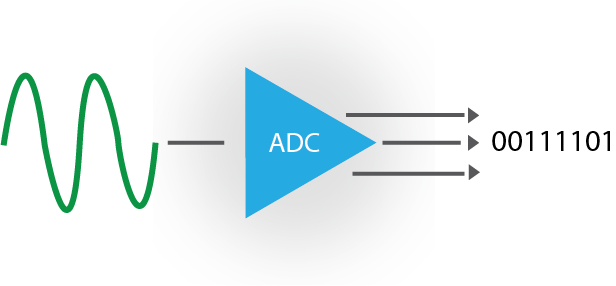
\includegraphics[width=10cm]{ADC-1.png}
\caption{Analog-to-Digital Converter Principle}
\label{fig:adc}
\end{figure}
\vspace*{0.1cm}

La série des STM32F4xx a jusqu'à trois ADCs chacun ayant jusqu'à 19 channels. 16 channels externes connectés aux I/O pins, et 3 internes.

\newpage

\subsubsection{Universal Asynchronous Receiver Transmitter}

L'UART est un protocol émetteur-récepteur asynchrone universel. Il permet la transmission de données d'un équipement A, ici un microcontrôleur STM32F4 à un équipement B, dans notre cas l'ordinateur. Les données à transmettre existent sous forme parallèle (octet(s)) et sont transmises sous forme série (Least Significant Bit en premier). Les données reçues sous forme série (LSB en premier ...) puis reconditionnées sous forme d'octet(s). Pour permettre une liaison plus rapide les données sont stockées dans un buffer (mémoire tampon) d'une capacité de 64 octets. 

\vspace*{0.1cm}
\begin{figure}[htb]
\centering
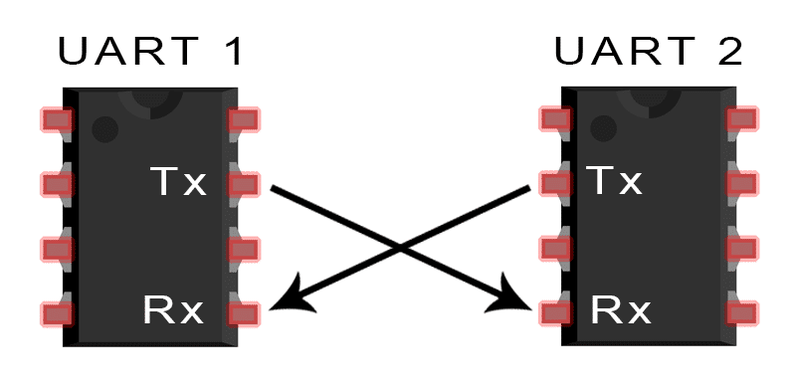
\includegraphics[width=10cm]{uart.png}
\caption{UART Protocol}
\label{fig:uartprotocol}
\end{figure}
\vspace*{0.1cm}

Entre deux équipements les fils sont croisés : Tx1 relié à Rx2 et Tx2 relié à Rx1. Dans notre cas nous utilisons l'USART (Synchrone) en mode asynchrone : aucune horloge (bit clock) n'est transmise entre l'emetteur et le récepteur. Le recepteur ignore le moment auquel il va recevoir une donnée. Afin de faciliter l'interopérabilité entre périphériques  des vitesses de transmission sont normalisées par multiples et sous-multiples de 9600 baud, l'unité baud correspondant à une vitesse de transmission de un bit par seconde.

\vspace*{0.1cm}
\begin{figure}[htb]
\centering
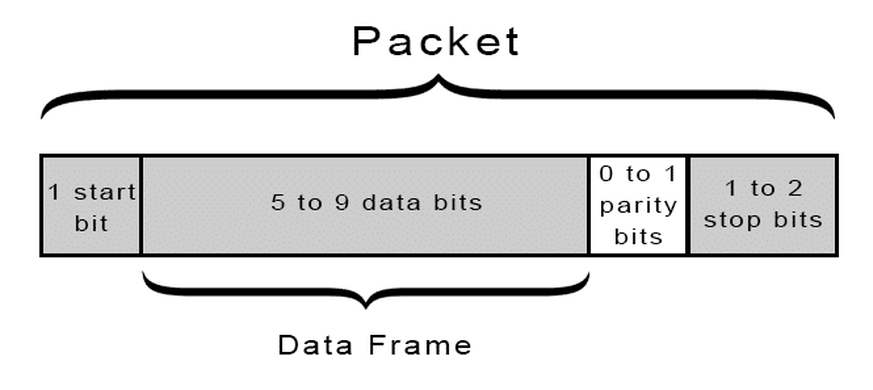
\includegraphics[width=10cm]{uartframe.png}
\caption{Trame UART}
\label{fig:uartframe}
\end{figure}
\vspace*{0.1cm}

\newpage

\subsection{Qt | Cross-Platform API}

\vspace*{0.1cm}
\begin{figure}[htb]
\centering

\includegraphics[width=5cm]{TheQtCompany_logo_1200x630.png}
\caption{Qt Logo}
\label{fig:qt}
\end{figure}
\vspace*{0.1cm}

Qt est une bibliothèque logicielle orientée objet (API) développée en \CC. Elle aspire principalement à être une plateforme de développement d’interfaces graphiques GUI (Graphical User Interface). Qt fournit un ensemble de classes décrivant des éléments graphiques (widgets) et des éléments non graphiques : accès aux données (fichier, base de données), connexions réseaux (socket), gestion du multitâche (thread), XML, etc.

Qt Creator est l’environnement de développement intégré dédié à Qt et facilite la gestion d’un projet Qt. Son éditeur de texte offre les principales fonctions que sont la coloration syntaxique, le complètement, l’indentation, etc… Qt Creator intègre en son sein les outils Qt Designer et Qt Assistant. Il intègre aussi un mode débuggage.

\newpage

\section{Développement}
Cette section traitera du développement du projet, du code mis en place et des choix faits pour mener à bien celui-ci. Le workflow sera présenté de façon chronologique, c'est à dire d'abord la récupération de la donnée via l'ADC, puis la transmission sur l'UART de la STM32, et enfin la réception et l'affichage via Qt.\\

\vspace*{0.1cm}
\begin{figure}[htb]
\centering
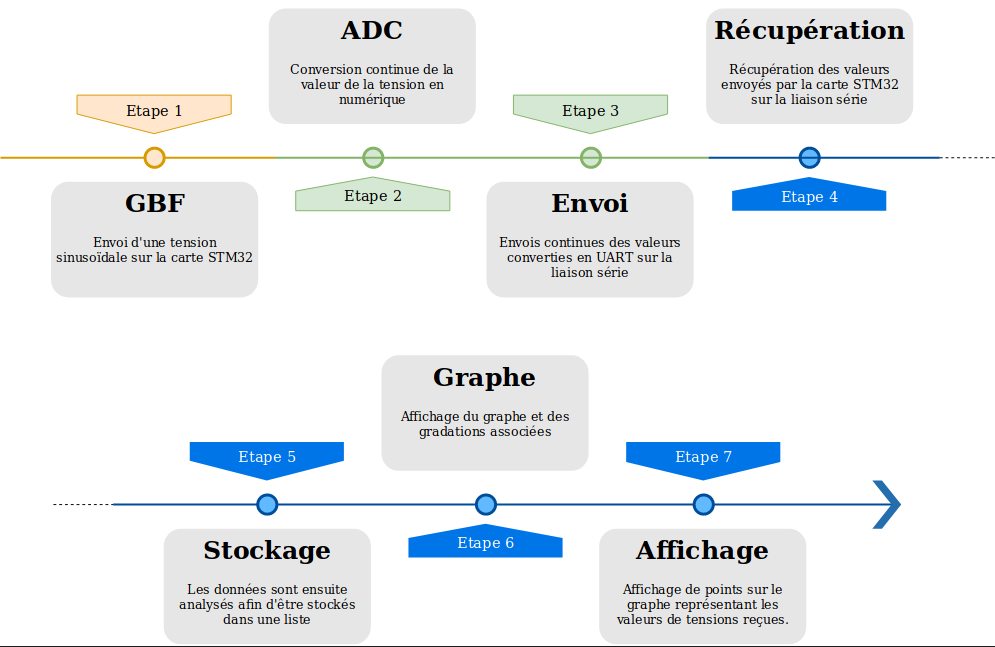
\includegraphics[width=17cm]{Workflow33.png}
\caption{WorkFlow}
\label{fig:workflow}
\end{figure}
\vspace*{0.1cm}

\newpage

\subsection{Récupération et Envoi}

On configure d'abord toutes les fonctions de la STM32 que l'on va utiliser : UART, Timer, ADC, GPIO.\\

Configuration ADC1, USART2, TIM2 :

\vspace{3mm}
\begin{lstlisting}
  hadc1.Instance = ADC1;
  hadc1.Init.ClockPrescaler = ADC_CLOCK_SYNC_PCLK_DIV2;
  hadc1.Init.Resolution = ADC_RESOLUTION_12B;
  hadc1.Init.ScanConvMode = DISABLE;
  hadc1.Init.ContinuousConvMode = ENABLE;
  hadc1.Init.DiscontinuousConvMode = DISABLE;
  hadc1.Init.ExternalTrigConvEdge = ADC_EXTERNALTRIGCONVEDGE_NONE;
  hadc1.Init.ExternalTrigConv = ADC_SOFTWARE_START;
  hadc1.Init.DataAlign = ADC_DATAALIGN_RIGHT;
  hadc1.Init.NbrOfConversion = 1;
  hadc1.Init.DMAContinuousRequests = DISABLE;
  hadc1.Init.EOCSelection = ADC_EOC_SINGLE_CONV;
\end{lstlisting}

\vspace{3mm}
\begin{lstlisting}
  huart2.Instance = USART2;
  huart2.Init.BaudRate = 115200;
  huart2.Init.WordLength = UART_WORDLENGTH_8B;
  huart2.Init.StopBits = UART_STOPBITS_1;
  huart2.Init.Parity = UART_PARITY_NONE;
  huart2.Init.Mode = UART_MODE_TX_RX;
  huart2.Init.HwFlowCtl = UART_HWCONTROL_NONE;
  huart2.Init.OverSampling = UART_OVERSAMPLING_16;
\end{lstlisting}

\vspace{3mm}
\begin{lstlisting}
  htim2.Instance = TIM2;
  htim2.Init.Prescaler = 1;
  htim2.Init.CounterMode = TIM_COUNTERMODE_UP;
  htim2.Init.Period = 15999;
  htim2.Init.ClockDivision = TIM_CLOCKDIVISION_DIV1;
  htim2.Init.AutoReloadPreload = TIM_AUTORELOAD_PRELOAD_DISABLE;
\end{lstlisting}
\newpage

On va récupérer par interruption une valeur de l'ADC à chaque fois qu'une période du timer s'est écoulée, puis on appliquera un masque sur cette valeur afin de ne garder que la partie qui nous intéresse pour la transmettre sur l'UART de cette façon :

\vspace{3mm}
\begin{lstlisting}
void HAL_TIM_PeriodElapsedCallback(TIM_HandleTypeDef *htim) {
	uint32_t value = HAL_ADC_GetValue(&hadc1);
	value &= 0x00000FFF;
	char buffer[10];
	sprintf(buffer, "%04d\n", value);
	HAL_UART_Transmit(&huart2, (uint8_t*)buffer, 5, 10);
	HAL_ADC_Start(&hadc1);
	HAL_TIM_Base_Start_IT(htim);
}
\end{lstlisting}

Le callback est appelé à chaque période écoulée.

\newpage

\subsection{Architecture global du programme C++}

Concernant le programme C++ chargé de la récupération des données sur le port série et de l'affichage "oscilloscope", nous avons divisé notre programme en différentes classes.

\vspace*{0.1cm}
\begin{figure}[htb]
\centering
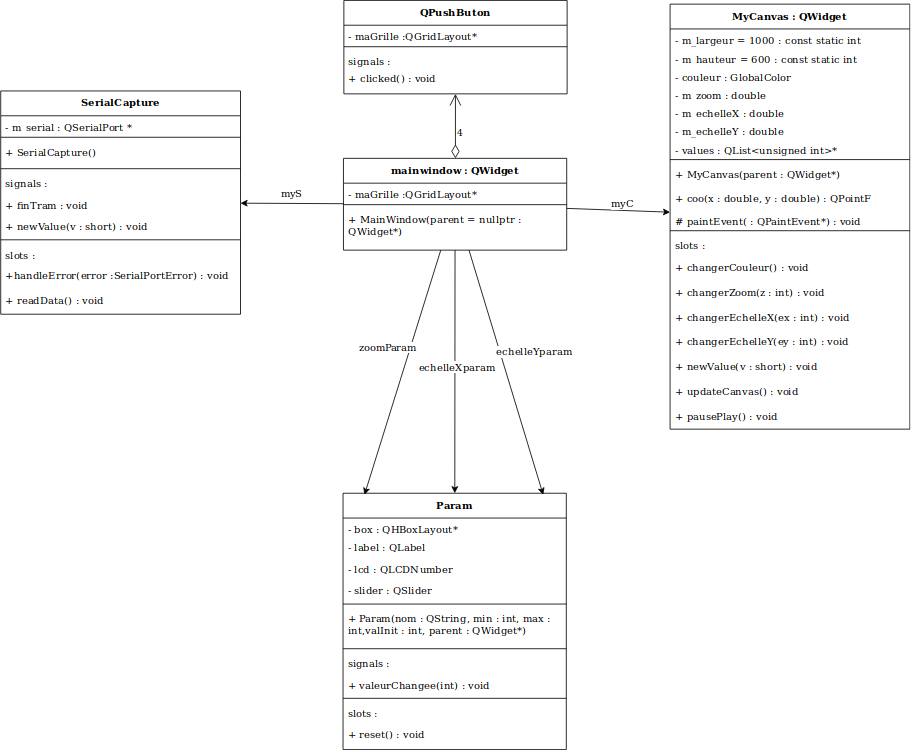
\includegraphics[width=17cm]{diagrammeclass.png}
\caption{Diagramme de Classes}
\label{fig:classdiag}
\end{figure}
\vspace*{0.1cm}

\newpage

Comme vu ci-dessus, on a \emph{mainwindow} qui est la classe qui représente la fenêtre globale du programme. Elle est composé de divers éléments. Tout d'abord, une grille contenant tous les différents boutons que nous allons mettre en place ; et le \emph{canvas} qui réprésente la partie "dessinée" sur l'affichage, c'est à dire le graphe. La classe \emph{mainwindow} va aussi contenir les différents sliders permettant de moduler l'affichage selon les désirs de l'utilisateur.\\

Les différents boutons mis en place sont : 

\begin{description}
    \item [ o Reset ] Remet la valeur des différents sliders par défaut.
    
    \item[ o Pause ] Arrêt de l'actualisation de l'affichage. C'est donc une mise en pause de l'affichage.
    
    \item[ o Couleur ] Change la couleur de la courbe.
    
    \item[ o Quitter ] Fermeture du programme\\

\end{description}

Les différents sliders permettant à l'utilisateur d'agir sur le graphe sont : 

\begin{description}
    \item[ o EchelleX / Y ] Modification de l'échelle de l'axe voulu
    \item[ o Zoom ] Zoom sur le graphe
\end{description}

\vspace*{0.1cm}
\begin{figure}[htb]
\centering
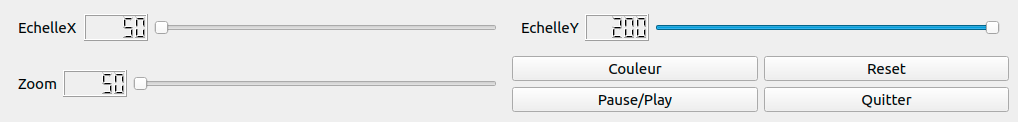
\includegraphics[width=17cm]{boutons.png}
\caption{Possibles interactions Homme-Machine}
\label{fig:slots}
\end{figure}
\vspace*{0.1cm}

Ensuite, parmi les classes importantes, il y a donc \emph{Canvas} qui permet de gérer toute la partie affichage du graphe, c'est à dire le graphe en lui-même mais aussi les axes et le quadrillage dans lequel s'affiche le graphe.\\

Et on a bien sur la classe \emph{SerialCapture} qui permet de gérer toute la partie réception des données via USB et stockage de ces données.

\newpage

\subsection{Réception et Affichage}

Ayant envoyé les données en Tx sur le port série, on récupère maintenant en Rx sur Qt grâce à la classe QtSerialPort. Voici comment on traite les données lues :

\vspace*{3mm}

\begin{lstlisting}
void SerialCapture::readData() {
    QByteArray buf=m_serial->readAll();
    std::string buffS = buf.toStdString();
    
    /* Decoupage de la longue tram recue a l'aide des \n */
    QList<QByteArray> laListe = buf.split('\n');

    /* Suppression des donnees qui pourraient etre troquees */
    laListe.pop_front();
    laListe.pop_back();

    /* Chaque valeur est emise par un signal */
    foreach (auto v, laListe) {
        std::cout<<"recu : "<<v.toStdString()<<std::endl;
        emit newValue(v.toShort());
    }
    emit finTram(); // Fin tram permet de mettre a jour le canvas une seul fois par lecture
}
\end{lstlisting}
\vspace{3mm}

Pour les afficher, on place maintenant nos widgets dans deux grilles dans notre mainWindow comme ci-dessous :

\vspace{3mm}
\begin{lstlisting}
    /*Creation de deux grilles pour y ranger nos widgets*/
    maGrille  = new QGridLayout(this);
    QGridLayout* maGrille2 = new QGridLayout();
    QGridLayout* grilleBoutons = new QGridLayout();

    myC = new MyCanvas(this);

    /*SerialCapture, responsable de la recuperation des donnees*/
    myS = new SerialCapture();
    connect(myS,&SerialCapture::finTram,myC,&MyCanvas::updateCanvas);
    connect(myS,&SerialCapture::newValue,myC,&MyCanvas::newValue);
\end{lstlisting}

\vspace{3mm}

On connectera ensuite nos param, boutons et sliders utilisés pour rendre le GUI ergonomique et agréable. L'architecture des connects est décrite en UML à la figure 6 ci-après, l'architecture générale des objets est décrite en UML à la figure 7.

\newpage

\vspace*{0.1cm}
\begin{figure}[htb]
\centering
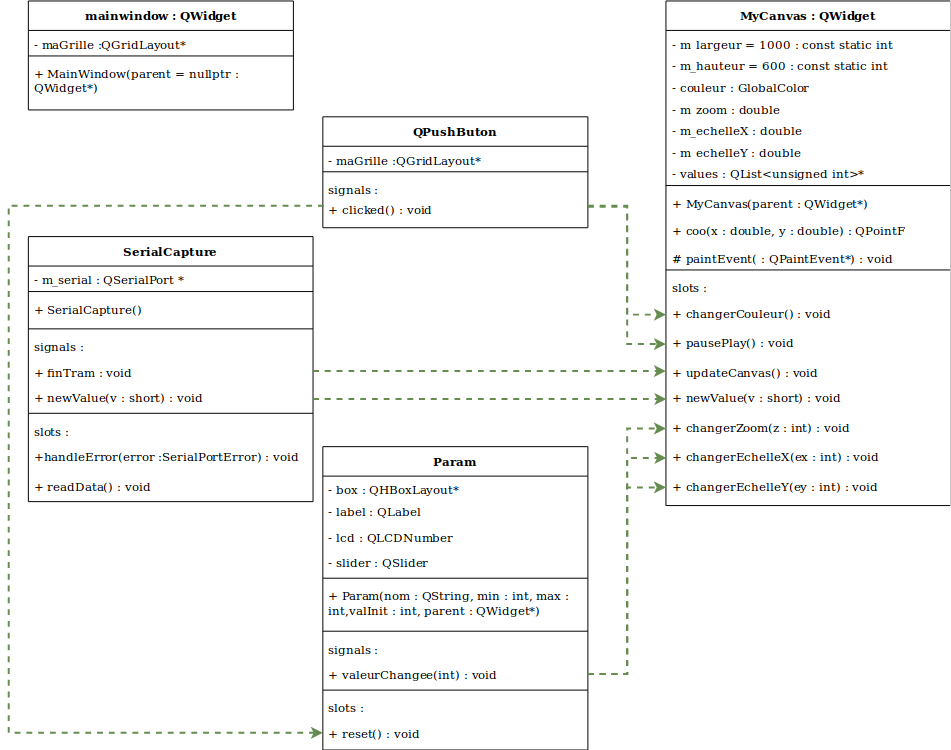
\includegraphics[width=17cm]{diagrammeconnect.png}
\caption{Diagramme des "Connects"}
\label{fig:classdiag}
\end{figure}
\vspace*{0.1cm}

\newpage

\subsubsection{Synchronisation de l'Affichage}

Le dernier objectif du programme est de, selon le désir de l’utilisateur, pouvoir gérer l’affichage de la courbe en fonction de la dernière courbe affichée, c’est à dire que la nouvelle courbe doit s’afficher alignée par rapport à l’ancienne courbe. \\

Il faut savoir que cet ajout s'est faît à la toute fin du délai permis pour le rendu du projet. Cette modification n'est donc pas visible sur différents documents présents sur ce rapport, notamment les diagrammes de classe et de connections ainsi que certaines captures d'écran.\\

L'ajout de cette fonctionnalité implique quelques modifications du programme, on va tout d’abord ajouter un bouton permettant d’activer ou de désactiver la synchronisation.\\ 

Afin de mettre en place cette synchronisation, on va en premier lieu enregistrer le premier point de l’affichage actuel. Ensuite, à la prochaine réception des valeurs de l’ADC, on va comparer chaque valeur à la valeur enregistrée afin d’obtenir un point proche et de la valeur sur laquelle s’effectue le trigger. Après avoir trouvé cette valeur, on enregistre toute les valeurs suivantes dans la liste values sur laquelle on s’appuie pour l’affichage des points. On obtient donc une liste des points à afficher qui commence à partir d’un point très proche du premier point de la dernière courbe affiché.\\ 

Lors du test de si la valeur de la liste est assez proche de la valeur enregistrée, on teste aussi le sens en regardant la prochaine valeur afin d’éviter de se synchroniser avec la partie de la courbe qui descend alors que l’on recherche un point de lorsque la courbe est montante.\\

Cette solution n’est pas parfaite, elle fonctionne avec certains types de courbes comme les sinusoïdes par exemple mais peut ne pas marcher avec des courbes un peu plus complexe où sur la même période on peut retrouver des parties de courbe qui se ressemblent.\\


\newpage

\section{Résultats}

Maintenant toute l'architecture décrite et le workflow explicité, on peut montrer les résultats de notre oscilloscope.

\vspace*{0.1cm}
\begin{figure}[htb]
\centering
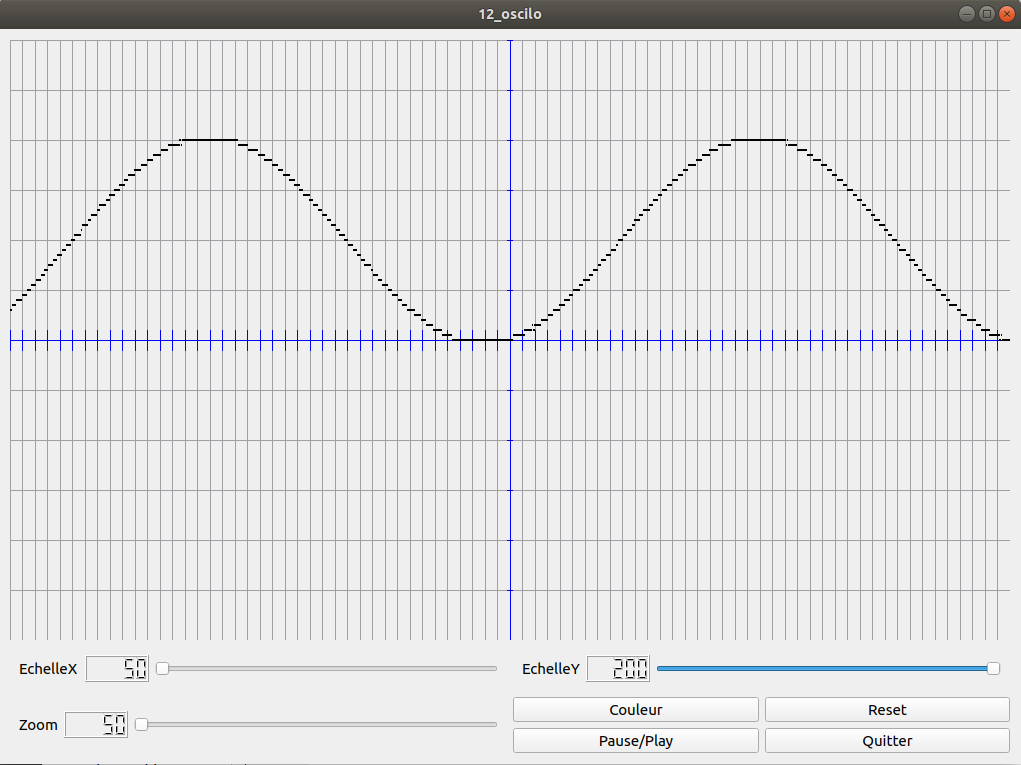
\includegraphics[width=14cm]{oscillo.png}
\caption{Oscillo on Qt}
\label{fig:oscillo}
\end{figure}
\vspace*{0.1cm}

Le programme permet d'augmenter l'echelle des abscisses avec EchelleX, des ordonnées avec EchelleY ( plus ou moins de points sur l'axe ). Le bouton zoom permet d'afficher plus ou moins de points sur notre grille. Le bouton couleur permet de changer la couleur de la courbe selon un set défini.
On voit que l'on a une belle sinusoïde, mais ce n'est pas tout, on a aussi été capable d'afficher des rampes de fréquences différentes, comme ci-dessous.

\newpage

\begin{figure}[htb]
\centering
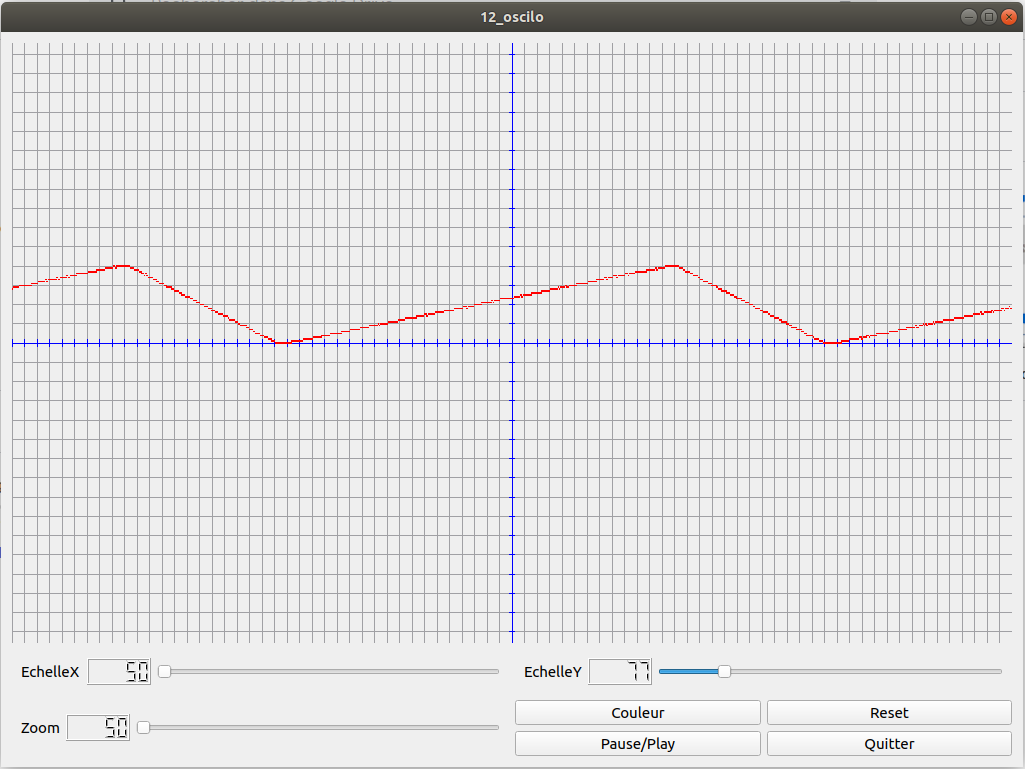
\includegraphics[width=10cm]{Rampe4ghz.png}
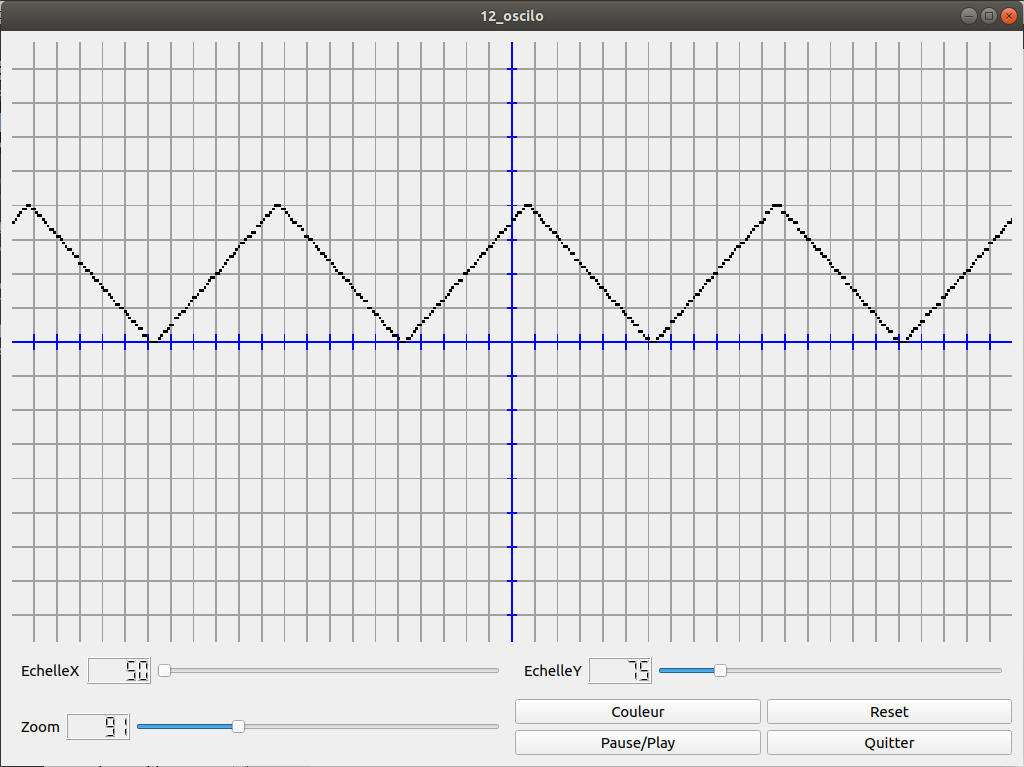
\includegraphics[width=10cm]{oscillotriangle.png}
\caption{Oscillo on Qt (Rampe 4HZ et 1HZ)}
\label{fig:rampe1}
\end{figure}
\vspace*{0.1cm}

Ici, on peut voir deux signaux rampes envoyés du GBF à deux fréquences différentes. En jouant avec les échelles, on pourrait changer la forme des signaux afin de d'observer une carastéristique précise de la courbe.



\newpage

\section{Conclusion}

Le projet nous a permis de mettre en place un visualiseur de signaux via Qt. Ce fut une première expérience concernant la cohabitation entre la carte STM32 et Qt. De par la récupération et le traitements des données données générées par la carte.\\

Ce projet s'est assez bien déroulé, nous n'avons pas connu de gros problèmes et nous avons eu une première version fonctionnelle assez vite. La difficulté s'est surtout situé au niveau des ajouts que l'on a fait par la suite. Notamment la synchronisation que l'on a décidé d'ajouter au dernier moment et donc que nous n'avons pas pu tester dans les meilleurs conditions.\\


\textbf{Projet :} \emph{https://github.com/LavergneC/Cpp-Osciloscope}

\end{document}